%插入样式内容
\documentclass[12pt]{article}
%%---------------------------------------------------------------------
% packages
% geometry
\usepackage{color}
\usepackage{geometry}
% font
\usepackage{fontspec}
\defaultfontfeatures{Mapping=tex-text}  %%如果没有它,会有一些 tex 特殊字符无法正常使用,比如连字符。
\usepackage{xunicode,xltxtra}
\usepackage[BoldFont,SlantFont,CJKnumber,CJKchecksingle]{xeCJK}  % \CJKnumber{12345}: 一万二千三百四十五
\usepackage{CJKfntef}  %%实现对汉字加点、下划线等。
\usepackage{pifont}  % \ding{}
% math
\usepackage{amsmath,amsfonts,amssymb}
% color
\usepackage{color}
\usepackage{xcolor}
\definecolor{EYE}{RGB}{199,237,204}
\definecolor{FLY}{RGB}{128,0,128}
\definecolor{ZHY}{RGB}{139,0,255}
% graphics
\usepackage[americaninductors,europeanresistors]{circuitikz}
\usepackage{tikz}
\usetikzlibrary{positioning,arrows,shadows,shapes,calc,mindmap,trees,backgrounds}  % placements=positioning
\usepackage{graphicx}  % \includegraphics[]{}
\usepackage{subfigure}  %%图形或表格并排排列
% table
\usepackage{colortbl,dcolumn}  %% 彩色表格
\usepackage{multirow}
\usepackage{multicol}
\usepackage{booktabs}
% code
\usepackage{fancyvrb}
\usepackage{listings}
% title
\usepackage{titlesec}
% head/foot
\usepackage{fancyhdr}
% ref
\usepackage{hyperref}
% pagecolor
\usepackage[pagecolor={EYE}]{pagecolor}
% tightly-packed lists
\usepackage{mdwlist}

\usepackage{styles/iplouccfg}
\usepackage{styles/zhfontcfg}
\usepackage{styles/iplouclistings}
\usepackage{listings} 
\usepackage{hyperref}
\usepackage{color,framed}
%\usepackage{styles/pythonhighlight}
%\usepackage{graphicx}
%%---------------------------------------------------------------------
% settings
% geometry
\geometry{left=2cm,right=1cm,top=2cm,bottom=2cm}  %设置 上、左、下、右 页边距
\linespread{1.5} %行间距
% font
\setCJKmainfont{Adobe Kaiti Std}
%\setmainfont[BoldFont=Adobe Garamond Pro Bold]{Apple Garamond}  % 英文字体
%\setmainfont[BoldFont=Adobe Garamond Pro Bold,SmallCapsFont=Apple Garamond,SmallCapsFeatures={Scale=0.7}]{Apple Garamond}  %%苹果字体没有SmallCaps
\setCJKmonofont{Adobe Fangsong Std}
% graphics
\graphicspath{{figures/}}
\tikzset{
    % Define standard arrow tip
    >=stealth',
    % Define style for boxes
    punkt/.style={
           rectangle,
           rounded corners,
           draw=black, very thick,
           text width=6.5em,
           minimum height=2em,
           text centered},
    % Define arrow style
    pil/.style={
           ->,
           thick,
           shorten <=2pt,
           shorten >=2pt,},
    % Define style for FlyZhyBall
    FlyZhyBall/.style={
      circle,
      minimum size=6mm,
      inner sep=0.5pt,
      ball color=red!50!blue,
      text=white,},
    % Define style for FlyZhyRectangle
    FlyZhyRectangle/.style={
      rectangle,
      rounded corners,
      minimum size=6mm,
      ball color=red!50!blue,
      text=white,},
    % Define style for zhyfly
    zhyfly/.style={
      rectangle,
      rounded corners,
      minimum size=6mm,
      ball color=red!25!blue,
      text=white,},
    % Define style for new rectangle
    nrectangle/.style={
      rectangle,
      draw=#1!50,
      fill=#1!20,
      minimum size=5mm,
      inner sep=0.1pt,}
}
\ctikzset{
  bipoles/length=.8cm
}
% code
\lstnewenvironment{VHDLcode}[1][]{%
  \lstset{
    basicstyle=\footnotesize\ttfamily\color{black},%
    columns=flexible,%
    framexleftmargin=.7mm,frame=shadowbox,%
    rulesepcolor=\color{blue},%
%    frame=single,%
    backgroundcolor=\color{yellow!20},%
    xleftmargin=1.2\fboxsep,%
    xrightmargin=.7\fboxsep,%
    numbers=left,numberstyle=\tiny\color{blue},%
    numberblanklines=false,numbersep=7pt,%
    language=VHDL%
    }\lstset{#1}}{}
\lstnewenvironment{VHDLmiddle}[1][]{%
  \lstset{
    basicstyle=\scriptsize\ttfamily\color{black},%
    columns=flexible,%
    framexleftmargin=.7mm,frame=shadowbox,%
    rulesepcolor=\color{blue},%
%    frame=single,%
    backgroundcolor=\color{yellow!20},%
    xleftmargin=1.2\fboxsep,%
    xrightmargin=.7\fboxsep,%
    numbers=left,numberstyle=\tiny\color{blue},%
    numberblanklines=false,numbersep=7pt,%
    language=VHDL%
    }\lstset{#1}}{}
\lstnewenvironment{VHDLsmall}[1][]{%
  \lstset{
    basicstyle=\tiny\ttfamily\color{black},%
    columns=flexible,%
    framexleftmargin=.7mm,frame=shadowbox,%
    rulesepcolor=\color{blue},%
%    frame=single,%
    backgroundcolor=\color{yellow!20},%
    xleftmargin=1.2\fboxsep,%
    xrightmargin=.7\fboxsep,%
    numbers=left,numberstyle=\tiny\color{blue},%
    numberblanklines=false,numbersep=7pt,%
    language=VHDL%
    }\lstset{#1}}{}
% pdf
\hypersetup{%pdfpagemode=FullScreen,%
            pdfauthor={Haiyong Zheng},%
            pdftitle={Title},%
            CJKbookmarks=true,%
            bookmarksnumbered=true,%
            bookmarksopen=false,%
            plainpages=false,%
            colorlinks=true,%
            citecolor=green,%
            filecolor=magenta,%
            linkcolor=cyan,%red(default)
            urlcolor=cyan}
% section
%http://tex.stackexchange.com/questions/34288/how-to-place-a-shaded-box-around-a-section-label-and-name
\newcommand\titlebar{%
\tikz[baseline,trim left=3.1cm,trim right=3cm] {
    \fill [cyan!25] (2.5cm,-1ex) rectangle (\textwidth+3.1cm,2.5ex);
    \node [
        fill=cyan!60!white,
        anchor= base east,
        rounded rectangle,
        minimum height=3.5ex] at (3cm,0) {
        \textbf{\thesection.}
    };
}%
}
\titleformat{\section}{\Large\bf\color{blue}}{\titlebar}{0.1cm}{}
% head/foot
\setlength{\headheight}{15pt}
\pagestyle{fancy}
\fancyhf{}

\chead{\color{black!50!green}Cifar10 And MNIST}

%\lfoot{\color{blue!50!green}Dai Jialun}
\cfoot{\color{blue!50!green}\href{http://vision.ouc.edu.cn/~zhenghaiyong}{CVBIOUC}}
\rfoot{\color{blue!50!green}$\cdot$\ \thepage\ $\cdot$}
\renewcommand{\headrulewidth}{0.4pt}
\renewcommand{\footrulewidth}{0.4pt}


%%---------------------------------------------------------------------
\begin{document}
%%---------------------------------------------------------------------
%%---------------------------------------------------------------------
% \titlepage
\title{\vspace{-2em} Cifar-10与MNIST训练集\\
\normalsize{}}
\author{Dai Jialun}
\date{\vspace{-0.7em} \today \vspace{-0.7em}}
%%---------------------------------------------------------------------
\maketitle\thispagestyle{fancy}
%%---------------------------------------------------------------------
\maketitle
%\tableofcontentsG
\section{Cifar10}
\subsection{Cifar10介绍}!
CIFAR-10数据集由10类总共60000张32$\times$32的彩色图像组成,其中每一类都有6000张图像。在60000张图像中,有50000张的训练图像与10000张的测试图像。如图Figure~\ref{fig:introduction}。

\begin{figure}[!ht]
\centering
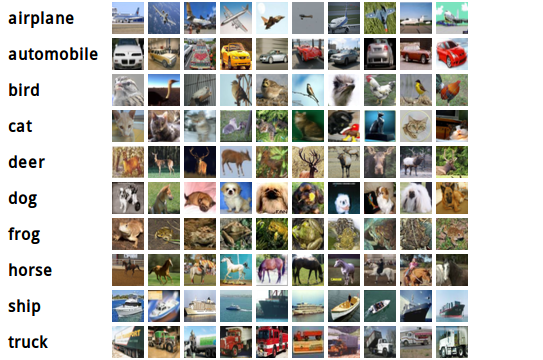
\includegraphics[width=0.6\textwidth]{cifar10}
\caption{Cifar10数据集}
\label{fig:introduction}
\end{figure}

数据集被分成5个训练组和1个测试组,每一组都有10000张图像。其中,测试组从10类中的每一类随机挑选出的1000张图像,即测试组中每一类图像数量相同。训练组从所剩下的图像中随机挑选,因此在某些训练组中,存在某一类中的图像可能比其他类图像多,即某个训练组中每一类图像数量可能不同。但是从整体上看,在5组训练组的合计中,每一类有5000张图像。

另外在数据集中,每一类的图像都是独立存在,不存在有一张图像在两个类别中出现的情况。


\subsection{Cifar10数据集版本与格式}
Cifar10数据集版本:
\begin{itemize}
\item CIFAR-10 python version
\item CIFAR-10 Matlab version
\item CIFAR-10 binary version (suitable for C programs)
\end{itemize}

{\color{blue} Python/Matlab版(cifar-10-batches-py / cifar-10-batches-mat):}

在这里介绍了数据集的Matlab版本。Python版本的结构与其是相同的。在下载的文档中,包含了{\scriptsize{data\_batch\_1}},{\scriptsize{data\_batch\_2}},{\scriptsize{data\_batch\_3}},{\scriptsize{data\_batch\_4}},{\scriptsize{data\_batch\_5}},以及{\scriptsize{test\_batch}}。在Matlab上加载后,每一个组文件将会生成一个包含以下文件的文件夹:%每一个文件都是由Python的``cPickle''所产生的pickled对象。下面是Python程序,会打开一个文件并且返回一个目录。

\begin{comment}
\begin{python}
def unpickle(file)
  Import cPickle
  fo=open(file,'rb')
  dict=cPickle.load(fo)
  fo.close()
  return dict
\end{python} 
\end{comment}


\begin{description}
\item[data] 一个类型为unit8的10000$\times$3072的numpy矩阵。已知每一张图像都是3通道,大小为32$\times$32。这个矩阵的每一行存储一个32$\times$32图像的3个不同通道的像素值。每一行表示一张图像,刚开始的1024列(32$\times$32)表示红色通道像素值,接下来的1024列(32$\times$32)表示绿色通道像素值,最后的1024列(32$\times$32)表示蓝色通道像素值。图像是行优先存储的。%因此,data数组刚开始的32是第一行图像的红色通道值。
\item[labels] 一个列表,一列包含了10000个数字,范围为0$\sim$9。在列表中,第$i$个数字表示在数组数据中,第$i$张图像的标注。
\end{description}

数据集包含了另外一个{\scriptsize{batches.meta}}文件。它也包含了一个对象,有以下内容:
\begin{description}
\item[label\_names] 一个含有10个目标的列表,其描述了标注数字对应具体的类别名字。例如,label\_names[0]=``airplane''
\end{description}


\begin{figure}[!ht]
  \centering 
  \subfigure[data]{ 
 %   \label{fig: } %% label for first subfigure 
    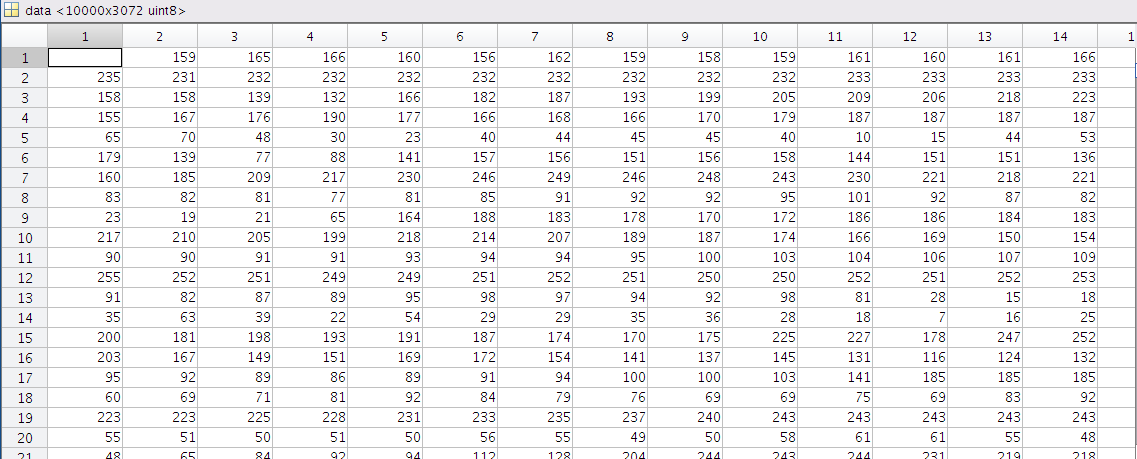
\includegraphics[width=0.6\textwidth]{data}} 
  \subfigure[labels]{ 
 %   \label{fig: result1: b} %% label for second subfigure 
    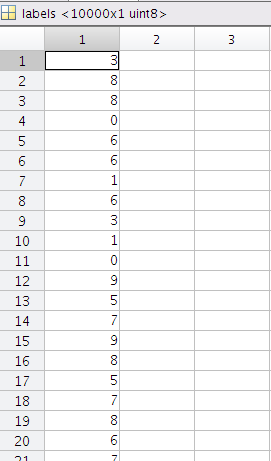
\includegraphics[width=0.14\textwidth]{labels}} 
  \caption{data\_batch\_1在Matlab下形式}
 % \label{fig: } %% label for entire figure 
\end{figure}


\begin{comment}
\begin{figure}[!ht]
\centering
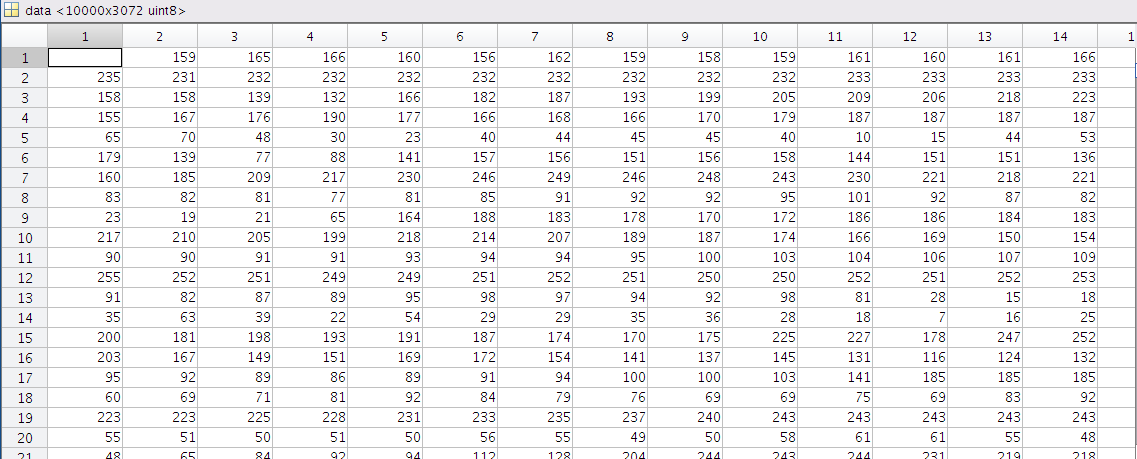
\includegraphics[width=0.5\textwidth]{data}
\caption{cifar10}
%\label{fig:framework}
\end{figure}

\begin{figure}[!ht]
\centering
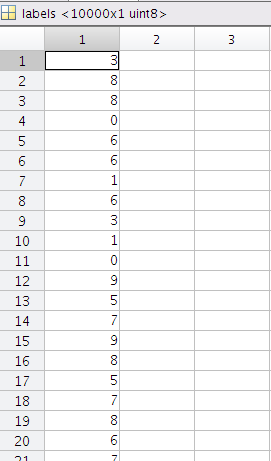
\includegraphics[width=0.2\textwidth]{labels}
\caption{cifar10}
%\label{fig:framework}
\end{figure}
\end{comment}


\begin{figure}[!ht]
\centering
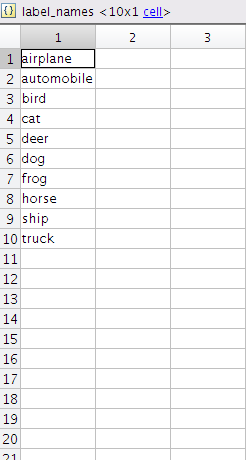
\includegraphics[width=0.2\textwidth]{label_name}
\caption{label\_name}
%\label{fig:framework}
\end{figure}

{\color{blue} 二进制版本的数据集(cifar-10-batches-bin):}

二进制版本包含了{\scriptsize{data\_batch\_1.bin}},{\scriptsize{data\_batch\_2.bin}},{\scriptsize{data\_batch\_3.bin}},{\scriptsize{data\_batch\_4.bin}},{\scriptsize{data\_batch\_5.bin}},以及{\scriptsize{test\_batch\_bin}}。在Caffe中,用{\footnotesize{get\_cifar10.sh}}自动获取的数据集就为二进制版本。每个文件的格式如下:

\colorbox{gray}{  
\vbox{  \scriptsize{
<1 $\times$ label> <3072 $\times$ pixel>

$\dots$

<1 $\times$ label> <3072 $\times$ pixel>  }
}}  

也就是说,刚开始的第一列是训练或测试图像的标注,是一个范围在0$\sim$9之间的数字。接下来的3072列是图像3通道的像素值。最前面的1024列(32$\times$32)是红色通道的像素值,接下来的1024列(32$\times$32)是绿色通道的像素值,最后的1024列(32$\times$32)是蓝色通道的像素值。这些值是按行优先排列的。

每一个文件包含10000个这样像3073列的图像行,即为形式为10000$\times$3073。

另外,还有一个 {\scriptsize{batches.meta.txt}}的文件。这是一个ASCII文件,表示0$\sim$9之间的数字对应的各个类别名字。这仅仅是一个含有10个类别名字的列表,每一个一行。

\begin{figure}[!ht]
  \centering 
  \subfigure[]{ 
 %   \label{fig: } %% label for first subfigure 
    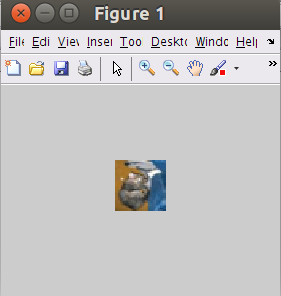
\includegraphics[width=0.29\textwidth]{first1}} 
  \subfigure[]{ 
 %   \label{fig: result1: b} %% label for second subfigure 
    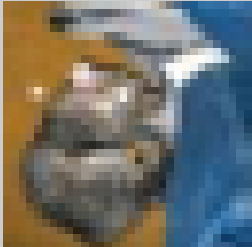
\includegraphics[width=0.31\textwidth]{first2}} 
  \caption{One image in Cifar10}
  \label{fig:origin} %% label for entire figure 
\end{figure}

在Cifar10数据集中,图像只以像素值形式的数据表示。如果要查看图像,需要经过程序的变换,转换成可打开与显示的图像格式。如图Figure~\ref{fig:origin}。



\section{MNIST}
\subsection{MNIST介绍}
MNIST数据集是手写数字图像,其训练集有60000张图像,测试集有10000张图像。这只是一个更大的数据集NIST的一个子集。这些数字图像已经经过尺寸的规范化与在图像的置中心处理。

这个数据集适合一些人想用学习技术以及模式识别方法来处理真实世界的数据,而且不需要花太多功夫在预处理和格式化方面的工作上。

这个数据集总共有4个文件:
\begin{itemize}
\item \textbf{{\footnotesize{train-images-idx3-ubyte.gz}}} {\footnotesize{training set images (9912422 bytes)}} 
\item \textbf{{\footnotesize{train-labels-idx1-ubyte.gz}}} {\footnotesize{training set labels (28881 bytes)}} 
\item \textbf{{\footnotesize{t10k-images-idx3-ubyte.gz}}} {\footnotesize{test set images (1648877 bytes)}} 
\item \textbf{{\footnotesize{t10k-labels-idx1-ubyte.gz}}} {\footnotesize{test set labels (4542 bytes)}}
\end{itemize}

在NIST中的手写数字图像,都为灰度保真图,而且经过规范化处理,图像大小为28$\times$28。

MNIST数据集是由NIST的Special Database 3 (SD3)和Special Database 1(SD1)所组成,二者包含了手写数字的二值图像。NIST中最初将SD-3作为训练集,SD-1作为测试集。然而,SD-3比SD-1更清晰,更容易识别。主要是因为SD-3是从Census Bureau的员工处收集的,而SD-1是从高中生处收集的。从学习实验中得出可靠的结论要求结果与训练集的选择无关,并且测试样本是完整数据集。因此,必须通过混合NIST数据集来建立一个全新的数据集。

MNIST训练集是由SD-3的30000张图像和SD-1的300000张图像组成。测试集是由SD-3的5000张图像和SD-1的5000张图像组成。训练集中所包含的图像是从大约250个人中收集到的。基本可以判定训练集与测试集的数字是不同的人所写的。

SD-1是由500个不同的人所写的58527张数字图像。在SD-1中,数据是杂乱无章地排列的。这个排列方式与SD-3不同,在SD-3中每个人所写的数字图像是按序列排列的。我们可用人工方法来分辨SD-1的数字图像由哪个人缩写。我们将SD-1分为两部分:由前250个人所写的数字图像放在训练集中,剩下的250个人所写数字放在测试集中。因此,我们有了两个子集,每个子集有大约30000张图像。新的训练集从SD-3中的\#0开始提取图像30000张图像,与之前SD-1中一个子集的30000张图像合并,组成一个60000张的训练集。与其相似,新的测试集是由SD-3中的\#35000开始提取图像,与之前SD-1中另一个子集的图像合并,组成一个大的测试图像。但是在这里只需要测试集中的10000张测试图像(从SD-1中的5000张图像和从SD-3中的5000张图像)。当然,60000张的训练图像也是完全可用的。


\subsection{MNIST数据库格式}

数据存储在一个用来存放向量和多维矩阵的文件格式中。MNIST数据库主要包含四个文件:{\footnotesize{train-images-idx3-ubyte.gz}},{\footnotesize{train-labels-idx1-ubyte.gz}},{\footnotesize{t10k-images-idx3-ubyte.gz}},{\footnotesize{t10k-labels-idx1-ubyte.gz}}。在Caffe中,用{\footnotesize{get\_mnist.sh}}自动获取的数据集就是上述形式。训练集包含了60000张图像,测试集包含了10000张图像。

\begin{figure}[!ht]
  \centering 
  \subfigure[]{ 
 %   \label{fig: } %% label for first subfigure 
    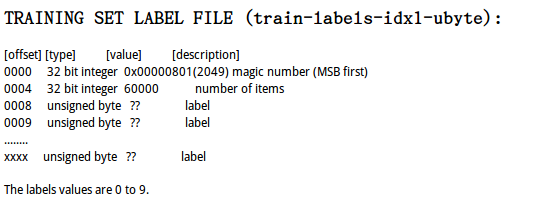
\includegraphics[width=0.31\textwidth]{mnist1}} 
  \subfigure[]{ 
 %   \label{fig: result1: b} %% label for second subfigure 
    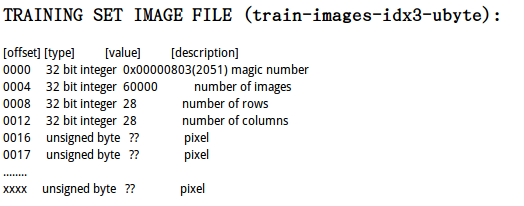
\includegraphics[width=0.3\textwidth]{mnist2}} 
  \caption{MNIST数据库训练集内容}
  \label{fig: } %% label for entire figure 
\end{figure}

在MNIST数据库中,图像数据以上述形式存储。如果要查看图像,需要经过程序的变换,转换成可打开与显示的图像格式。如图Figure~\ref{fig:mnist}。
\begin{figure}[!ht]
  \centering 
  \subfigure[]{ 
 %   \label{fig: } %% label for first subfigure 
    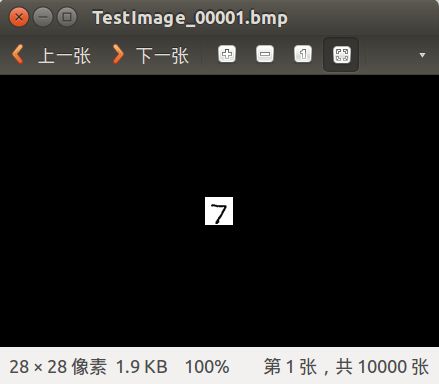
\includegraphics[width=0.3\textwidth]{mnist_example1}} 
  \subfigure[]{ 
 %   \label{fig: result1: b} %% label for second subfigure 
    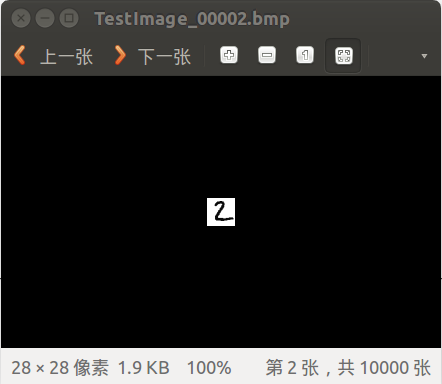
\includegraphics[width=0.3\textwidth]{mnist_example2}} 
  \caption{One image in MNIST}
  \label{fig:mnist} %% label for entire figure 
\end{figure}
%%---------------------------------------------------------------------
\end{document}
